\newpage
\section{Auswertung}
\label{sec:Auswertung}
Die gesamte Auswertung wird mit Hilfe der Bibilotheken \cite{matplotlib}, \cite{numpy}, \cite{scipy} und
\cite{uncertainties} in \textit{python} durchgeführt. \\
Berechnungen aus nebeneinander liegenden Temperaturen, geteilt durch die Zeitdifferenz ihrer Aufnhame von \SI{30}{\second}
ergeben eine Heizrate $h$ von \SI{1.015(6)}{\kelvin\per\minute} beziehungsweise von \SI{1.734(19)}{\kelvin\per\minute}.
Die Polarisation der Probe findet bei \SI{322.95}{\kelvin} und einem angelegtem Feld von \SI{900}{\volt} statt.

\subsection{Untergrund}
\label{sec:Unter}
Für die Bestimmung des Untergrunds $I(T)$ werden die Messdaten links und rechts neben dem betrachteten Bereich,
welcher durch zwei senkrechte violette Linien begrentzt ist, 
herangezogen. Diese sind in den Abbildungen \ref{fig:Messdaten1} und \ref{fig:Messdaten2} grün dargestellt.
Desweiteren ist auch der Fit der Form
\begin{equation}
    \label{eqn:exp}
    I(T) = a \cdot \exp \left(b\cdot T \right) + c
\end{equation}
in den Abbildungen \ref{fig:Messdaten1} und \ref{fig:Messdaten2} eingezeichnet.
Die Parameter für die Heizrate von etwa \SI{1}{\kelvin\per\minute} ergeben sich zu
\begin{align*}
    a &= \SI{0.20(7)e-11}{\ampere} \\
    b &= \SI{0.019(11)}{\per\kelvin} \\
    c &= \SI{-0.03(7)e-11}{\ampere}.
\end{align*}
Und für die Heizrate von etwa \SI{2}{\kelvin\per\minute} auf
\begin{align*}
    a &= \SI{0.82(12)e-11}{\ampere} \\
    b &= \SI{0.018(4)}{\per\kelvin} \\
    c &= \SI{-0.30(11)e-11}{\ampere}.
\end{align*}
Für die folgenden Rechnungen wird dieser Untergrund den Messwerten abgezogen.
\begin{figure}[htb]
  \centering
  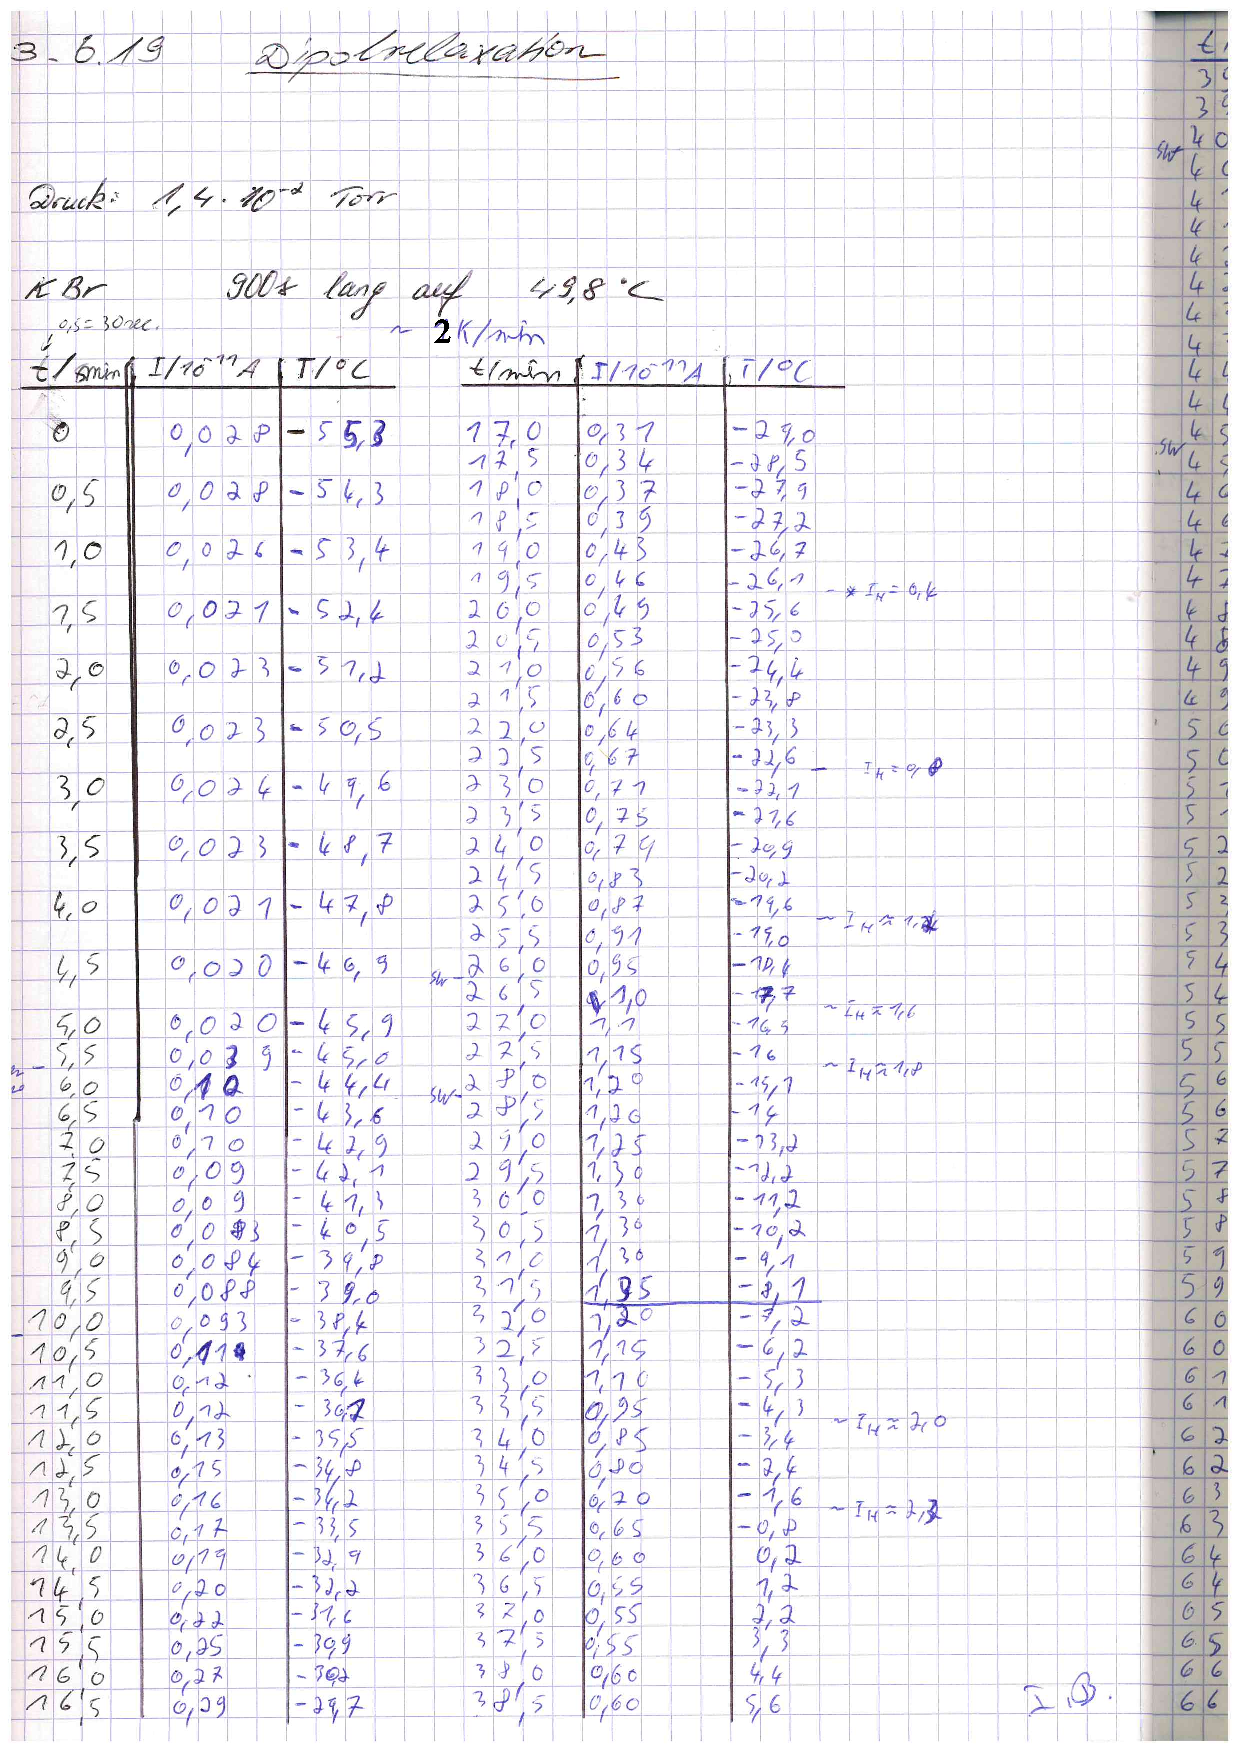
\includegraphics[width=\textwidth]{build/Messdaten1.pdf}
  \caption{Die Messdaten für eine Heizrate von etwa \SI{1}{\kelvin\per\minute}. Nicht verwendete Messdaten sind blau und die für den Untergrund verwendeten grün dargestellt. Die violetten Linien makieren den betrachtete Bereich, die Orange das Maximum.}
  \label{fig:Messdaten1}
\end{figure}
\begin{figure}[htb]
  \centering
  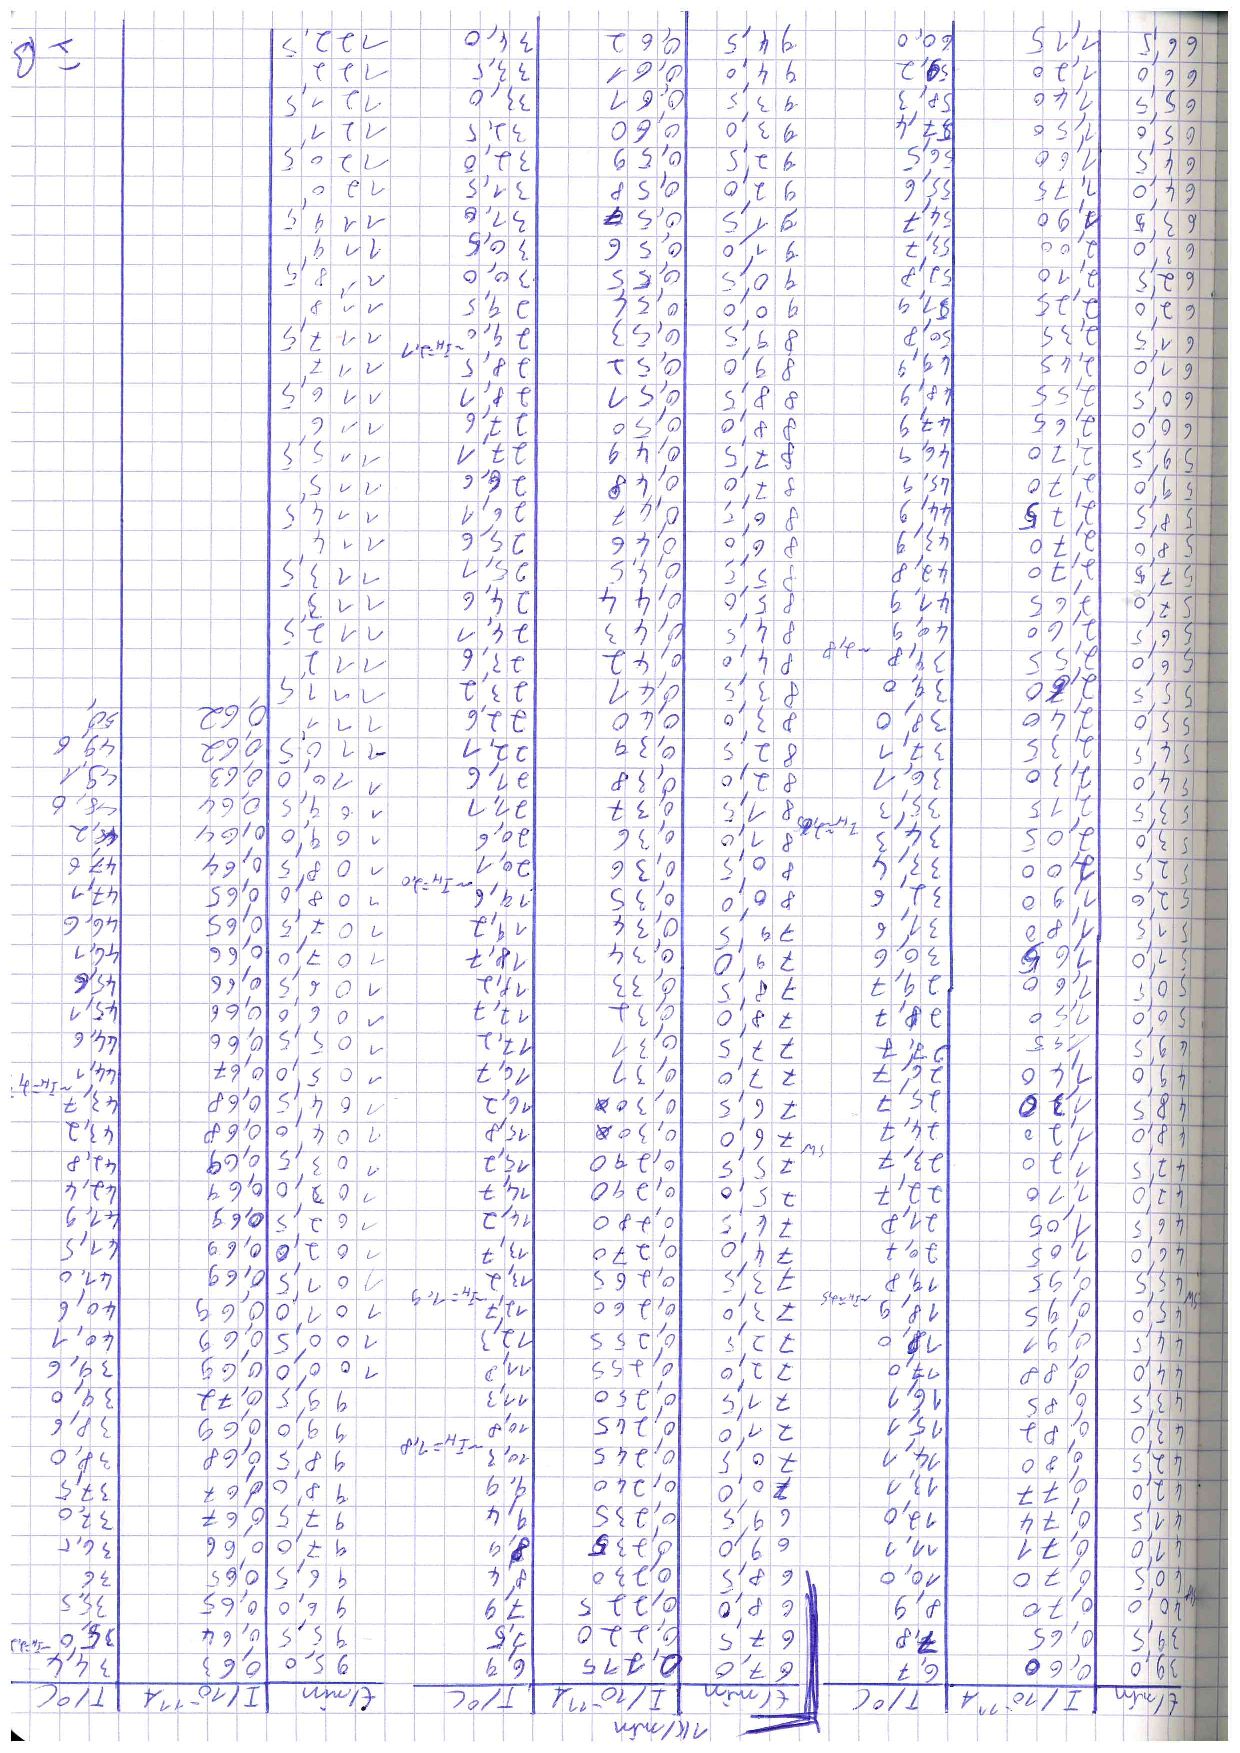
\includegraphics[width=\textwidth]{build/Messdaten2.pdf}
  \caption{Die Messdaten für eine Heizrate von etwa \SI{2}{\kelvin\per\minute}. Nicht verwendete Messdaten sind blau und die für den Untergrund verwendeten grün dargestellt. Die violetten Linien makieren den betrachtete Bereich, die Orange das Maximum.}
  \label{fig:Messdaten2}
\end{figure}
\FloatBarrier

\subsection{Stromdichteansatz}
\label{sec:klT}
Zur Berechnung der Aktivierungsenergie $W$ bei kleinen Temperaturen werden die Daten vom linken Rand des betrachteten Bereichs bis zum Maximum, welches durch die senkrechte orange Linie gekennzeichnet ist,
aus den Abbildungen \ref{fig:Messdaten1} und \ref{fig:Messdaten2} verwendet. Es wird die Näherung der Stromdichte für kleine Temperaturen
herangezogen. Der gemessene Strom $i(T)$ ist dabei bis auf einen konstanten Faktor proportionel zur Stromdichte. Der Strom wird logarithmiert
und in Abhängigkeit von der reziproken Temperatur $\frac{1}{T}$ in Abbildung \ref{fig:klT} aufgetragen. Für jede Heizrate erfolgt eine lineare Ausgleichsrechnung der Form
\begin{equation}
    \label{eqn:lin}
    \ln\left(\frac{i(T)}{\SI{1e-11}{\ampere}}\right) = -\frac{W}{\symup{k_B} T} + \text{const} = \frac{a}{T} + b,
\end{equation}
mit der Boltzmann-Konstante $\symup{k_B} = \SI{1.380649e-23}{\joule\per\kelvin}$ \cite{codata}, welche ebenfalls in Abbildung \ref{fig:klT} zusehen ist.
Es können die Parameter zu
\begin{align*}
    a_1 &= \SI{-822(28)e1}{\kelvin} \\
    b_1 &= \num{31.9(11)} \\
    a_2 &= \SI{-112(6)e2}{\kelvin} \\
    b_2 &= \num{43.5(24)}
\end{align*}
bestimmt werden.
Somit lassen sich die Aktivierungsenergien $W_\text{i} = -a_\text{i} \cdot \symup{k_B}$ zu
\begin{align*}
    W_1 &= \SI{1.13(4)e-19}{\joule} \\
    W_2 &= \SI{1.54(8)e-19}{\joule}
\end{align*}
bestimmen.
\begin{figure}[htb]
  \centering
  \includegraphics[width=\textwidth]{build/kleineT.pdf}
  \caption{Die verwendeten Messdaten bei kleinen Temperaturen für den Stromdichteansatz bei den beiden Heizraten und der dazugehörigen Ausgleichsgeraden.}
  \label{fig:klT}
\end{figure}
\FloatBarrier

\subsection{Polarisationsansatz}
\label{sec:grT}
Nun wird die Relaxationszeit $\tau_0$ sowie die Aktivierungsenergie auf Grundlage des Polarisationsansatzes bestimmt.
Hierzu werden die Daten zwischen den beiden senkrechten violetten Linien in den Abbildungen \ref{fig:Messdaten1} und \ref{fig:Messdaten2} verwendet.
Dazu wird eine numerische Integration der Form
\begin{equation}
    \label{eqn:int}
    \int_T^{T^*} |i(T')| \symup{d}\,T'
\end{equation}
durchgeführt. Dies erfolgt mit \textit{Scientific Python} \cite{scipy} und der Trapez-Regel. Dabei ist zu beachten, dass $i(T^*) \approx \SI{0}{\ampere}$ gelten muss.
Die lässt sich für die Heizrate von etwa \SI{1}{\kelvin\per\minute} auf $T^*_1 = \SI{275.85}{\kelvin}$ und für die Heizrate von etwa \SI{2}{\kelvin\per\minute} 
auf $T^*_2 = \SI{280.95}{\kelvin}$ approximieren, da diese den kleinsten absoluten Abstand zu \SI{0}{\ampere} haben.
Wird nun
\begin{equation*}
    ln\left(\frac{\int_T^{T^*} |i(T')| \symup{d}\,T'}{h_i \cdot |i(T)|}\right)
\end{equation*}
gegen $\frac{1}{T}$ aufgetragen und eine lineare Ausgleichrechnung der Form
\begin{equation}
    \label{eqn:lin2}
    ln\left(\frac{\int_T^{T^*} |i(T')| \symup{d}\,T'}{h_i \cdot |i(T)|}\right) = \frac{W}{\symup{k_B} \cdot T} + ln(\tau_0) = \frac{a}{T} + b
\end{equation}
durchgeführt, lässt sich aus dem Parameter $a$ die Aktivierungsenergie und aus dem Parameter $b$ die Relaxationszeit $\tau_0$ bestimmen.
Die in Abbildung \ref{fig:grT1} gezeigte Ausgleichsgerade ergibt die Parameter
\begin{align*}
    a_1 &= \SI{994(9)e1}{\kelvin} \\
    b_1 &= \num{-36.9(3)},
\end{align*}
wobei nur die Werte zwischen \SIrange{37.6e-4}{42.4e-4}{\per\kelvin} für die Ausgleichsrechnung herangezogen werden. Dabei ergibt sich
\begin{align*}
    W_1 &= \SI{1.372(12)e-19}{\joule} \\
    \tau_{0,1} &= \SI{9(3)e-17}{second}.
\end{align*}
Für die Heizrate von etwa \SI{2}{\kelvin\per\minute} ergeben sich diese Werte zu
\begin{align*}
    a_2 &= \SI{1124(29)e1}{\kelvin} \\
    b_2 &= \num{-41.6(11)} \\
    W_2 &= \SI{1.55(4)e-19}{\joule} \\
    \tau_{0,2} &= \SI{9(10)e-18}{second},
\end{align*}
dabei beschränkt sich der betrachtete Bereich auf \SIrange{36.8e-4}{42.0e-4}{\per\kelvin}.
\begin{figure}[htb]
  \centering
  \includegraphics[width=\textwidth]{build/großeT1.pdf}
  \caption{Werte zur Bestimmung der Relaxationszeit und der Aktivierungsenergie nach dem Polarisationsansatzes für die Heizrate von etwa \SI{1}{\kelvin\per\minute}.}
  \label{fig:grT1}
\end{figure}
\begin{figure}[htb]
  \centering
  \includegraphics[width=\textwidth]{build/großeT2.pdf}
  \caption{Werte zur Bestimmung der Relaxationszeit und der Aktivierungsenergie nach dem Polarisationsansatzes für die Heizrate von etwa \SI{2}{\kelvin\per\minute}.}
  \label{fig:grT2}
\end{figure}

\subsection{Relaxationszeit}
\label{sec:relax}
Des Weiteren lässt sich aus der Position des Maximums auch die Relaxationszeit $\tau_0$ nach
\begin{equation}
    \label{eqn:tau0}
    \tau_0 = \frac{\symup{k_B}T_\text{max}^2}{W \cdot h} \exp\left(-\frac{W}{\symup{k_B}T_\text{max}} \right)
\end{equation}
bestimmen. Dabei wird für $T_\text{max}$ das Maxiumum der geweiligen Heizrate nach Abzug des Untergrunds bestimmt.
Für die Aktivierungsenergie $W$ wird der gemittelte Wert für die jeweilige Heizrate aus beiden Verfahren verwendet.
Für die Heizrate von $h_1=\SI{1.015(6)}{\kelvin\per\minute}$, der gemittelten Aktivierungsenergie $W_1 = \SI{1.235(20)e-19}{\joule}$ und dem 
Maximum bei einer Temperatur von $T_\text{max, 1} = \SI{255}{\kelvin}$ ergibt sich die Relaxationszeit $\tau_{0,1} = \SI{2.5(15)e-15}{\second}$. 
Für die Heizrate $h_2=\SI{1.734(19)}{\kelvin\per\minute}$, der gemittelten Aktivierungsenergie $W_2 = \SI{1.55(5)e-19}{\joule}$ und dem 
Maximum bei einer Temperatur von $T_\text{max, 2} = \SI{260.95}{\kelvin}$ ergibt sich die Relaxationszeit $\tau_{0,2} = \SI{0.8(10)e-18}{\second}$.

% \subsection{Unterkapiel}
% \label{sec:Unterkapitel}

% \begin{figure}[htb]
%   \centering
%   \includegraphics[width=\textwidth]{Plot.pdf}
%   \caption{Bildunterschrift}
%   \label{fig:Plot1}
% \end{figure}
\FloatBarrier